\chapter{Introduction}

%-------------------------------------------------------------------------------------------------------

\section{Background}

\noindent
Path planning is a complex robotics task that scientists have been working on for several decades now \cite{DIJKSTRA, D*}. It is the classic problem of how to get from point A to B in the most efficient manner with an autonomous agent given a goal in an environment that can contain obstacles. One solution to this is grid-based path planners, algorithms designed specifically to solve this task by representing the environment using a grid of cells. Consider the way chess pieces travel across the board their movement is bound by cells, grid-based path planners work much in the same way. In this project we hope to establish a ranking among several path planners based on their overall efficiency. \\ 

\noindent
In May 2014 we as part of a team submitted an undergraduate third year thesis at the Institute of Technology Blanchardstown \cite{JMD14}. The goal contained within this thesis was to construct an autonomous rover capable of navigating and mapping an indoor environment. The robot would use several internal sensors connected to an Arduino microcontroller to collect data about its physical surroundings, this information would then be processed on a host PC and from it a real-time map would be created. Based on the layout of this map the robot would then be expected to safely navigate its way through the environment continuously. \\

\noindent
Overall this project fell short of its intended goal and many of the envisioned features remained unimplemented. The robot's behaviour was limited to simply mapping an environment during tele-operation. In all the final result left much to be desired. The flaw of this otherwise successful project was that it aimed to achieve too much, robotic navigation is based on the principle of three operating layers: 

\begin{enumerate}
\item Simultaneous Localisation and Mapping (SLAM)
\item Path Planning
\item Obstacle Avoidance
\end{enumerate}

\noindent
In the previous project we attempted to implement layers 1 and 2, unfortunately this proved too much given the time available and we ended with a layer 1 implementation. It is therefore one of the goals of this project to finish what had been previously started and address the path planning aspect of autonomous robotics. Path planning can be referred to as a \textit{global} solution which looks at the entire environment when it builds its path. Layer 3 is \textit{local} planning, it is used in cases where replanning is not feasible due to a sudden change. For the purposes of this primarily research based project we will be referring to layer 2 navigation exclusively. \\

\noindent
In this thesis we shall go on to discuss the concept of path planning in detail under our Literature Review where we will refer to several current approaches to grid based planning. After that we define the system that shall be used to test our hypothesis both virtually on a computer system and physically using a robotic platform. The implementation section covers how we went about realising our design, we then undertake a number of tests, and perform an analysis of the results. Lastly we conclude by objectively answering our hypothesis for this entire research project in the Conclusion. 

\newpage

%-------------------------------------------------------------------------------------------------------

\section{Motivation}

\noindent
The motivation for this project was driven by the shortcomings of the last project \cite{JMD14} that we were involved in. In \cite{JMD14} the objective was to build a fully autonomous robot capable of actively mapping and navigating its environment. Unfortunately this goal proved unrealistic given the time and resources available to the team, and due to the high learning curve and low-end hardware only the mapping functionality was implemented. Essentially this project is being driven by the failure of its predecessor, however this time it is not limited to just the implementation but also the analysis of robotic path planners and their effectiveness.

\begin{figure}[htbp]

\center \includegraphics[width=350pt]{illustrations/third_year}\\
\caption{In the previous project we performed a number of tests based on the robot's mapping functionality \cite{JMD14}.} 
\label{Third Year}

\end{figure}

\noindent
Another issue that we noticed during our initial research into path planners for robotic systems was the amount of choice when it came to algorithms. Each planner claimed to be that little be better than another by being faster at planning or producing shorter paths. Selecting the ``best'' planner can be incredibly difficult for a newcomer as up until now there has been no detailed comparison of these planners. Documenting how some of the most popular planners perform against each other will not only provide us with a valuable insight but also countless other newcomers to robotic navigation. 

\newpage

%-------------------------------------------------------------------------------------------------------

\section{Research Question(s)}

\noindent
The primary research question of this project is a follows:

\begin{center}
\textbf{To establish proportionally which is more significant with regard to path planning, faster computation times, or shorter path traversals.} \\
\end{center}

\noindent
By answering this research question what we are hoping to establish is what produces overall the best solution, a planner that computes paths that are suboptimal at a faster rate, or a planner that spends more time computing potentially shorter paths. When we think about the efficiency of a computer program we generally think in terms of time but with robotics we have to consider both the time spent in the processor and the physical movement. Answering this research question will tell us what is more expensive in the long run, extra computations, or more time spent traversing. \\

\noindent
The project will also aim to address the following additional research questions:

\begin{itemize}
\item What advances to date have been made in navigation systems for mobile robots?

\item How important is navigation with respect to robotics?

\item Will it be possible to develop a generic navigation system that is independent from the hardware architecture for mobile robots?

\end{itemize}

%-------------------------------------------------------------------------------------------------------

\newpage

\section{Objectives}

\noindent
Along side our research questions we have a set number of objectives that we aim to achieve by the end of this project. These objectives are as follows:

\begin{itemize}
\item To produce a literature review covering the advancements in autonomous navigation in robotic systems.

\item To develop and test a generic hardware independent navigation system for ground based mobile robots. 

\item To evaluate the effectiveness of path planning techniques in known environments. 

\item To assess the benefits of faster planning times against path traversal lengths.

\item To test the solution against a set of predefined challenges and evaluate its performance.

\end{itemize}

\newpage

%-------------------------------------------------------------------------------------------------------

\section{Feasibility}
\noindent
This project is being supervised by Prof. Arnold Hensman who has spent at least 3 years working in the research area and has supervised past projects in robotics including one that the candidate participated in \cite{JMD14}. It will build upon the work of a past project \cite{JMD14} which supports the hypothesis that autonomous navigation can be implemented with similar resources. The project has well defined requirements, milestones, deliverables, and the purposed candidate has already spent over a year working in the research area. \newline

\noindent
Most of the technical resources required to achieve this project's goals are already available, including a code base, all other required equipment such as a high quality laser range finder are on order. Two separate robotic systems with the core functionality needed to implement the purposed system already exist and are ready for development (Figure: \ref{Figure: Robot Platforms.}). 
\newline

\begin{figure}[htbp]

\center 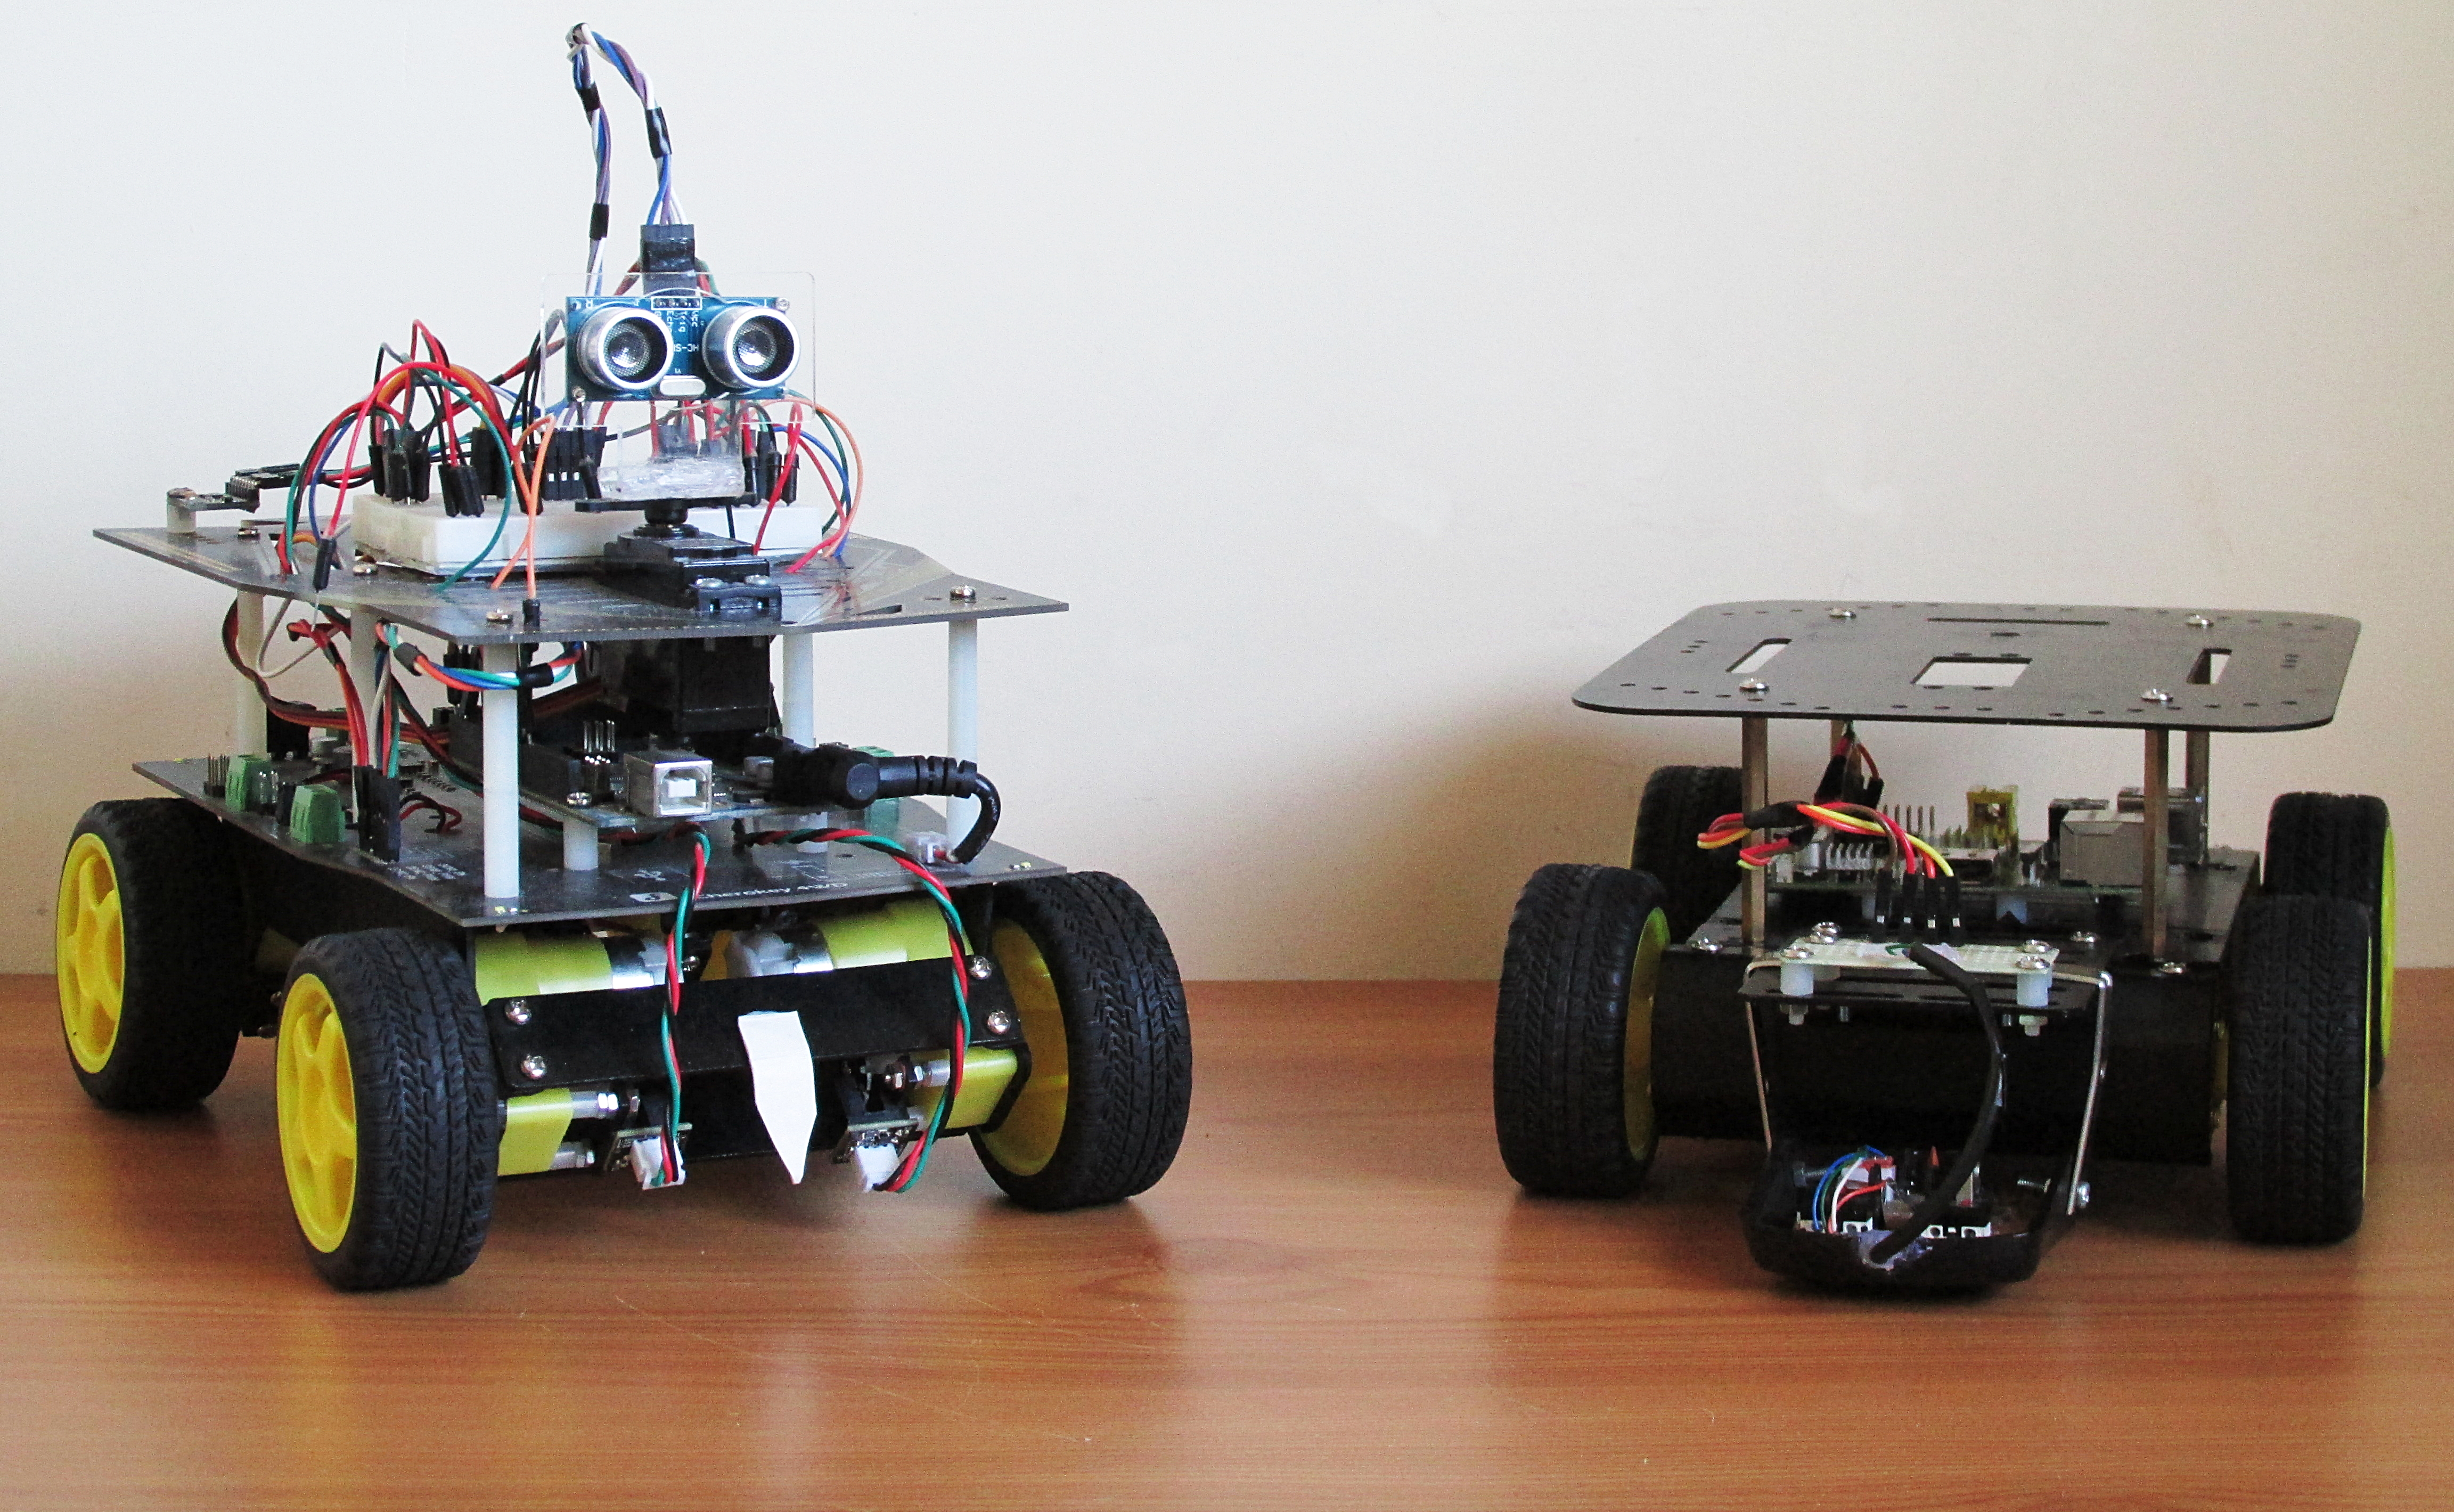
\includegraphics[width=230pt]{illustrations/robots}\\
\caption{The candidate's Cherokey robot and ITB's Pirate platform.} 
\label{Figure: Robot Platforms.}

\end{figure}
